%basic bad features, semantics. classes. lookup. overloading.
%- outline section 2 (matlab language)

\lstset{
basicstyle=\footnotesize\ttfamily, 
otherkeywords={>>},
keywordstyle=\ttfamily\bfseries,
numbers=none,
commentstyle=\color{blue}\sffamily\itshape,
stringstyle=\color{black}\ttfamily 
} 

In this chapter we describe key \matlab semantics and features to provide
necessary background for compiler writers and tool developers to understand
\matlab and its challenges, and to motivate our approach of constructing a
``tame" intermediate representation and \matlab callgraph.  In each section
we give a description followed by annotated examples using the \matlab
read-eval-print loop.   In the examples, ``\lstinline{>>}" indicates a line of
user input,  and the following line(s) give the printed output.

\section{Basics}

\matlab was originally designed in the 1970s to give access to features of {\sc
FORTRAN} (like {\sc Linpack}, {\sc Eispack}) without having to learn {\sc
FORTRAN}\cite{MatlabOrigins}. As the name \smatlab \hspace{1pt} (MATrix LABoratory)
suggests, \matlab is centered around numerical computation. Floating point
matrices are the core of the language.  However, the language has evolved
beyond just simple matrices and now has a type system including matrices of
different types, compound types including cell arrays and structs, and function
references. 

Given its origins, \matlab is a language that is built around matrices. Every
value is a \textit{Matrix} with some number of dimensions, so every value has
an associated array shape. Even scalar values are $1 \times 1$ matrices.
Vectors are either $1 \times n$ or $n \times 1$ matrices and strings are just
vectors of characters.  

\matlab supports imaginary components for all numerical values, and almost all 
operators and library functions support complex inputs.

\begin{lstlisting}
>> a = [1, 2, 3; 4, 5, 6] % defining a matrix ...
 a =
     1     2     3
     4     5     6
>> size(a)                % ... which is a 2x3 matrix
     2     3
>> size(3)                % the scalar 3 is a 1x1 matrix
     1     1
>> size([1 2 3])          % a 1x3 vector - note how the MATLAB syntax does not require a comma
     1     3
>> size([5; 6; 7; 8; 9])  % a 5x1 vector
     5     1
>> size('hello world')    % a string, which is a 1x11 vector
     1    11
>> ['a' 'b'; 'e' 'f']     % a 2-dimensional matrix of characters
     ab
     ef
>> 3 + 2i                 % the imaginary part of a complex number is defined using i or j
     3.0000 + 2.0000i
\end{lstlisting}


\section{\matlab Operators}
\label{sec:operators}

\matlab includes a set of builtin operators. Besides the usual comparison 
(\lstinline{==}, \lstinline{>}, \lstinline{>=}, etc.) and logical
(\lstinline{&}, \lstinline{&&}, etc.) operators, \matlab includes a set of
numerical operations, most of which are defined for matrices.

\begin{lstlisting}
>> true | false            % a scalar logical operation - the result 'true' is shown as '1'
     1
>> [2 3 5] > [3 4 2]       % comparison operators operate on matrices
     0     0     1
>> [1 2; 0 3] & [2 3; 4 0] % logical operators operate on matrices
     1     1
     0     0
\end{lstlisting}

\matlab's 
operators work on matrices, but are overloaded to operate with scalar
arguments as well. In that case, operations are performed
element-wise.  This means that although \matlab treats scalars just as
$1 \times 1$ matrices, their semantics with respect to operations are
actually different from non-scalar matrices.

\subsection{Array vs Matrix Operators}
\label{sec:ArrayVsMatrix}

\matlab has two kinds of numerical operators, matrix operators and 
array operators. Matrix operators operate on whole matrices at once
(unless an argument is a scalar). These include the matrix multiplication (\lstinline{*}),
and matrix division (\lstinline{\}, \lstinline{/}).

Array operators always operate on matrices in an element-wise way. For example the 
array multiply operator {\tt .*} will multiply two matrices element by element.
Generally, if there exists an matrix and an array version of an operator, then the 
array version will have a \lstinline{.}-prefix (e.g \lstinline{*} vs \lstinline{.*}).

An exception to this is the conjugate transpose operator \lstinline{'}. Here, the corresponding
\lstinline{.'}-operator will compute the non-conjugate transpose.

\begin{lstlisting}
>> [1 1; 2 2] * [1 0; 0 2]  % the multiplication operator performs matrix multiplication
     1     2
     2     4
>> [1 1; 2 2] * 2           % with a scalar argument, it will perform an element-wise multiplication
     2     2
     4     4
>> [1 1; 2 2] == 2          % comparison/logical operators also support mixing of matrices and scalars
     0     0
     1     1
>> [1 1; 2 2] .* [1 0; 0 2] % the same matrices as above, but using array multiply
     1     0
     0     4
>> [3 i; 0 1+i]'            % conjugate transpose
     3       0          
     -1i     1-1i
>> [3 i; 0 1+i].'           % non-conjugate transpose
     3       0          
     1i      1+1i
\end{lstlisting}




\subsection{The Colon Operator}

A special operator is the colon-operator. It allows the creation of
vectors containing numeric ranges:

\begin{lstlisting}
>> 2:10 % the colon operator creates numerical ranges
     2     3     4     5     6     7     8     9    10
>> 2:3:10 % an optional middle operand defines a stepsize
     2     5     8
>> 5:-1:0 % the stepsize can also be negative
     5     4     3     2     1     0
\end{lstlisting}

The colon operator is most often used in for loops to iterate over numerical
ranges. This means that a \matlab for loop is actually a for-each loop,
using a colon operator will semantically create the range as an array:

\begin{lstlisting}
>> for i = 1:3; disp(i); end % iterate over a range-vector
     1
     2
     3
>> for i = 'foo'; disp(i); end % iterate over the characters of a string
     f
     o
     o
\end{lstlisting}


\subsection{Indexing Operators}

\matlab includes three indexing operators, '{\tt ()}', '{\tt \{\}}' and '{\tt .}'.
The {\tt ()}-operator is used for array indexing of variables, and for calling functions.
Some of the implications of this ambiguity is further discussed in section \secref{sec:lookup}.
The {\tt \{\}} indexing operator is used to index into cell arrays, which are
discussed in \secref{sec:cell}. The dot operator is used to reference structures
(see \secref{sec:struct}) and user-defined classes using the new syntax (see \secref{sec:newClasses})

The \matlab indexing operators are versatile. They support indexing using
scalars, and indexing using arrays. Multi-dimensional arrays can be indexed
using fewer dimensions than the array actually has, in which case the last
dimension will combine all remaining dimensions. It is also possible to index
using logical values. Using a colon ({\tt :}) will expand the whole dimension.
The special keyword {\tt end} is an expression that returns the last index of a dimension.


\begin{lstlisting}
>> a = [1 2 3; 4 5 6]; % creating a matrix
>> a(2,2) % indexing using scalar indices
     5
>> a(4) % indexing using fewer dimensions - the dimensions get collapsed
     5
>> a(1:2,1) % indexing using an array - created using the colon-operator
     1
     4
>> a(2,[3 2 1]) % indexing using an explicit array
     6     5     4
>> a(1,:) % a colon will expand the whole dimension
     1     2     3
>> a(a > 2) % indexing using a logical array - created by the expression a > 2
     4
     5
     3
     6
>> a(2,end-1) % using end to refer to the last but one element of a dimension
     5
\end{lstlisting}



\subsection{Operators vs Builtin Functions}
\label{sec:OpVsFn}

\matlab's operators are naturally builtin to the language. Besides the operators, 
\matlab provides additional builtin operations as functions. There are
a large number of builtin functions, going into the hundreds, that are
intrinsic to \matlab.  For scientists and engineers these are part of
the appeal of \matlab as a language. 

Besides the syntax, there is
little difference between operators and builtin functions. In fact,
operators are just syntactic sugar for functions that denote the same
operation, every operator has a corresponding function. For example,
using the operator
\lstinline{+} is equivalent to calling the function \lstinline{plus}.

Even the indexing operations are represented by builtin functions.
All three indexing operators ({\tt ()}, {\tt \{\}} and {\tt .}) are
represented by the function {\tt subsref} and {\tt subsasgn}, where the former one
is used to represent indexing operations on the left-hand side, and the latter 
is used to represent indexing operations on the right-hand side.
Because each function can represent different kinds of indexing operations,
\matlab will internally add more arguments to the indexing functions
to represent the extra information required. This is transparent to the user,
unless one wishes to overload indexing operations. Overloading is introduced in
\secref{sec:functions}.


\section{\matlab Type System}

\matlab is dynamically typed - variables need not be declared, they will
take on any value that is assigned to them.  Every \matlab value has
an associated \matlab class (henceforth we will use the name
\textit{mclass} when referring to a \matlab class, in order to avoid
confusion with the usual notion of a class).  The mclass generally denotes the 
type of the elements of a value.  For example, the mclass of an array of doubles
is {\tt double}.  The default numeric mclass is {\tt double}. While
\matlab also includes integer types, all numeric literals are doubles.

\begin{lstlisting}
>> n = 1          % the input literal and the output look like an integer
     1
>> class(n)       % however the mclass is is really double, the default 
     double
>> class(1:100)   % the mclass of the vector [1, 2, ..., 100] is double 
     double
\end{lstlisting}

\matlab has a set of builtin mclasses, which can be summarized as
follows: 
\begin{itemize}
     \item {\tt double}, {\tt single}: floating point values
     \item {\tt uint8}, {\tt uint16}, {\tt uint32}, {\tt uint64},
  {\tt int8}, {\tt int16}, {\tt in32}, {\tt int64}: integer values
     \item {\tt logical}: boolean values
     \item {\tt char}: character values (strings)
     \item {\tt cell}: inhomogeneous arrays
     \item {\tt struct}: structures
     \item {\tt function handle}: references to functions
\end{itemize}

Given that by default any numerical value in \matlab is a 
{\tt double}, all values that are intended to be of a different
numeric type have to be specifically converted. This also means that
when combining a value of some non-double mclass with a value
that is a {\tt double}, the result will be of the non-double 
mclass. This leads to the surprising semantics that adding an {\tt integer}
and a {\tt double} results in an {\tt integer}, because that is the more
specialized type.

\begin{lstlisting}
>> x = 3; y = int8(5);   % assign to x and y,  y is explicitly an integer
>> class(x)              % the class of x is double
     double
>> class(y)              % the class of y is int8
     int8
>> class(x+y)            % the result of x+y is int8,  not double
     int8
\end{lstlisting}




\section{\matlab Functions and Overloading}
\label{sec:functions}

A \matlab function is defined in a \texttt{.m} file which has the same name as
the function.\footnote{In the case where the name of the file and the function
do not match, the name of the file takes precedence.} So, for example,  a
function named \texttt{foo} would be defined in a file \texttt{foo.m},  and
that file needs to be placed either in the current directory, or in a directory
on the \matlab path. A function thus defined is called a \textbf{primary function}.
A \texttt{.m} file can also define \textbf{subfunctions}
following the main (primary) function definition in a file,  but those
subfunctions are only visible to the functions within the file.
Inside functions it is possible to define \textbf{nested functions},
which are visible only to the parent function.
Functions may also be defined in a \texttt{private/}
directory. These \textbf{private functions} are visible only to
functions defined in the parent directory.

\matlab allows overriding operations and functions to
operate on specific mclasses.  This is accomplished by defining the
function in a file inside a specially named directory which starts with
the character \texttt{@} followed by the name of the mclass.  For
example, one could create a specialized function \texttt{firstWord}
defined for Strings, by creating a file {\tt @char/firstWord.m}
somewhere on the \matlab path. Functions that are specialized in such a
way are called \textbf{overloaded functions}.


Overloaded functions have precedence over non-overloaded functions, but they do not have
precedence over nested functions, subfunctions (defined in the same file)
or private functions (defined in the \texttt{/private} directory).  So,
in our example, if there existed two definitions of {\tt firstWord.m},
one general implementation somewhere on the \matlab path, and one
overloaded implementation in a directory \texttt{@char} on the \matlab
path,  then a call to {\tt firstWord} with a {\tt char} argument will
result in a call to {\tt @char/firstWord.m}, whereas a call with an
argument with any other mclass,  will result in a call to the general
{\tt firstWord.m} definition. The lookup semantics are discussed in detail in \secref{sec:lookup}.

When calling a function that has overloaded versions with
multiple arguments of different mclasses, \matlab has to resolve which
version of the function to call. There doesn't exist a standard inheritance
relationship between the builtin mclasses. Rather, \matlab has the
notion of a \textbf{superior} or \textbf{inferior} class.   We were
unable to find a succinct summary of these relationships, so we generated a
\matlab program which exercised all cases and which produced a
\texttt{.dot} file describing all relationships, with all transitive
relationships removed.  \figref{Fig:Superior} shows the relationships
between different builtin mclasses, showing superior classes above
inferior classes. Note that some mclasses have no defined relationship.
For example, there are no defined inferior/superior relationships
between the different integer mclasses.
Further, note that {\tt double}, being the default mclass, is inferior to
integer mclasses. Also, the compound mclasses (\lstinline{struct} and 
\lstinline{cell}), are superior to all matrix mclasses.

\begin{figure}[htbp]
\begin{center}
\includegraphics[width=5.2in]{Figures/builtinClassRelationships.eps}
\caption{Superior/inferior class relationships for \matlab}
\label{Fig:Superior}
\end{center}
\end{figure}


When resolving a call with multiple arguments, \matlab finds the most
superior argument, and uses its mclass to resolve the call. If multiple
arguments have no defined superior/inferior relationships, \matlab uses
the leftmost superior argument. The argument which is used to resolve
an overloaded function is called the \textbf{dominant argument}.
For example, if a function is called
with three arguments with the mclasses ({\tt double}, {\tt int8}, {\tt
uint32}), in that order, then the second argument is the dominant argument, 
and \matlab attempts to find an overloaded version
for mclass {\tt int8}. If none is found, \matlab attempts to find a
non-overloaded version.

As previously mentioned, using an operator (like \lstinline{+}) is equivalent
to calling the corresponding function (\lstinline{plus} in this case).
So if the function corresponding to an operator is overloaded, it also means
that the operator will be overloaded. This allows overloading of \matlab operators.

The overloading semantics for \matlab means that if one intends
to build a complete callgraph, i.e. resolve all possible call edges,
one has to find all possible \matlab classes for all arguments, and one must
safely approximate the lookup semantics of functions, including the correct
lookup of overloaded functions using the mclass and the superior/inferior
mclass relationships from \figref{Fig:Superior}.

\section{\matlab Classes }

It is important to note that the mclass of a value does not completely
define its type.  For example, numeric \matlab values may be real or
complex, and all values have an array shape.  Both of these properties are
defined orthogonally to the notion of its mclass. Although a computation can
ask whether a value is complex or real,  and can ask for the shape of
an array,  the lookup semantics solely depend on the mclass, which
is effectively just a name.   Within the \matlab language, there is no
dedicated class of values to represent mclasses. Usually, strings
(char vectors) are used to denote mclasses. For example,
\lstinline{ones(3,2,'single')}, will call the builtin function 'ones'
and create a $3 \times 2$ array of unit values of mclass \texttt{single}.

\section{Function Handles}
\label{sec:lambda}

\matlab values with mclass {\tt function\_handle} store a reference to a
function. This allows passing functions as arguments to other
functions. Function handles can either be created to
refer to an existing function, or an anonymous function created by a lambda expression.
Lambda expressions may also encapsulate state from the
current workspace via free variables in the lambda expression.

\begin{lstlisting}
>> f = @sin              % a function handle to a named function
f = @sin
>> g = @(x) exp(a*x)     % a lambda with a free variable "a"
g = @(x)exp(a*x)
\end{lstlisting}

Function handles, and especially lambdas, are
useful in numerical computing, for example when calling numerical
solvers, as illustrated below.

\begin{lstlisting}
f = @(t,y) D*t + c; % set up derivative function
span = [0 1];       % set interval
y0 = [0:0.1:10]';   % set initial value
result = ode23s(f,span,y0); % use MATLAB library function to solve ODE
\end{lstlisting}

When building a callgraph of a program that includes function handles,
one needs to propagate function handles through the program
interprocedurally in order to find out which variables may refer to
function handles, and to find associated call edges.


\section{Compound Types}

\matlab has two builtin compound types. These are of mclass \lstinline{struct} and
\lstinline{cell}, respectively.

\subsection{Cell Arrays}
\label{sec:cell}

In \matlab, every value of an array needs to have the same mclass. A
cell array is an array of values that do not necessarily need to have
the same mclass, allowing inhomogeneous arrays. Also note that for a numerical array,
every element is necessarily a scalar. So cell arrays allows creating arrays
of matrices with different sizes.

\begin{lstlisting}
>> {1, 'hello world'}               % cell arrays allows bundling values with different types
    [1]    'hello world'
>> {[1 2 3], [3; 4; 5]}              % ...or values with just different shapes
    [1x3 double]    [3x1 double]    
>> {[1 2 3], 3, [3 4; 3 5]}         % cell arrays may contain any value,
    [1x3 double]    [3]    [2x2 double] 
>> {[1 2 3], 3, {1, 'hello world'}} % ...including other cell arrays
    [1x3 double]    [3]    {1x2 cell}
\end{lstlisting}

A cell array is semantically an array of cells (everything is an
array). A cell is a scalar value of class \lstinline{cell} that
contains some \matlab value. Array indexing (using
{\tt ()}) will give back cells, cell indexing (using {\tt \{\}}),
will return the values contained in the cells.

\begin{lstlisting}
>> c = {1, [1 2 3], 'hello world'}  % when creating a cell array
 c = 
    [1]    [1x3 double]    'hello world'
>> c(1)                             % array indexing will return the cell
    [1]
>> c{1}                             % whereas cell indexing will return the contained value
     1
>> [c; {0}, {2, 'foo'}]             % cells and cell arrays can be combined with array operators
    [1]    [1x3 double]    'hello world'
    [0]    [         2]    'foo'        
\end{lstlisting}

\subsection{Structures}
\label{sec:struct}

Structures are \matlab values of mclass {\tt struct}, and allow bundling of different
\matlab values. But unlike cell arrays, which are indexed by numbers, \rednote{structures} are indexed
by field names (i.e. Strings). Structures can be created simply by
accessing them using the dot-operator. elements can be read or written
using he dot-operator. Nested structures are allowed. \matlab also allows accessing
structs using strings - so the field names of a struct may not be know statically.

\begin{lstlisting}
>> s.a = 4 % structs are created by assigning into them
s = 
    a: 4

>> s.b = 'hello world' % new fields are created on the fly
s = 
    a: 4
    b: 'hello world'
>> s.a % elements are read and written using the dot-operator
    4
>> s.t.v = 4 % structs may contain any value, including other structs
s = 
    a: 4
    b: 'hello world'
    t: [1x1 struct]
>> s.t 
    v: 4
>> s.('foo') = true % it is possible to use strings as fieldnames
s = 
      a: 4
      b: 'hello world'
      t: [1x1 struct]
    foo: 1
\end{lstlisting}

If one wants to build a complete callgraph, which requires the
resolution of overloaded functions, one needs to know any possible
mclass for all values. This means that for structures and cell arrays,
we need to know what possible values are contained in them. Since both
structures and cell arrays can be accessed with index-values (numbers
of cell arrays, strings for structures) that are not statically known, and since both of
them may contain values of different mclasses, we may not be able to
estimate one exact mclass when a program retrieves a value out of a
structure or cell array. A static compiler has to either be able to
deal with incompletely typed programs (i.e. union types), or restrict
the semantics of \matlab to disallow such cases.


\section{Function Parameters and Arguments }

\matlab uses call-by-value semantics,  so that each parameter denotes a fresh
copy of a variable.\footnote{Actual \matlab implementations only make copies
where actually necessary, using either lazy copying when writing to an array
with reference count greater than 1, or by using static analyses to determine
where to insert copies\cite{CC2011}.}  This simplifies interprocedural
analyses for static compilation as calling a function cannot directly modify
local variables in the caller.

In \matlab, function arguments are  optional.  That is, when calling a function
one may provide fewer arguments than the function is declared with.  However,
\matlab does not have a declarative way of specifying default values, nor does
it automatically provide default values. That is, a parameter corresponding to
an argument that was not provided will simply be unassigned and a runtime error
will be thrown if an unassigned variable is read. 

\matlab does provide the function {\tt nargin} to query how many
arguments have been provided to the currently executing function. This allows
the programmer to use the value of nargin to explicitly assign values to the
missing parameters, as illustrated below.

\begin{lstlisting}
function [result1, result2] = myFunction(arg1,arg2)
   if (nargin < 1)  
     arg1 = 0;
   end
   if (nargin < 2)
     arg2 = 1;
   end;
   ...
end
\end{lstlisting}

As shown above, \matlab also supports assigning multiple return
variables. A function call may request any number of return values
simply by assigning the call into a vector of lvalues. Just like the
function arguments, the return values don't all need to be assigned,
and a runtime error is thrown if a requested return value is not
assigned. \matlab provides the {\tt nargout} function to query how
many results need to be returned.

Clearly a static compiler for \matlab must deal with optional arguments in a
sound fashion.



\section{\matlab User-Defined Classes}
\label{sec:classes}

A combination of the notion of overloaded functions and structures directly leads to \matlab's
user-defined mclasses. User defined mclasses are structures which have a user-defined
mclass attribute defining the class name. Overloaded functions for that class name act
as methods. Members are accessed like a structure.

Using the function overloading semantics, mclasses are defined in a directory whose name is the
class name, with a prefixed @-symbol. For example, we may want to define a mclass
{\tt polynom} to represent polynomials. We would define it in a directory {\tt @polynom/} somewhere
on the path.

\subsection{Constructors}

Similar to other object-oriented languages, a constructor is a function that returns
an object of some class. In \matlab, constructors are defined in the directory where the class
resides and have the same name as the class. So in our example, the constructor would be defined
in some file {\tt @polynom/polynom.m}. Note that in order to lookup this function, \matlab
does not use overloading semantics - {\tt polynom} can be called with arbitrary arguments, 
and will refer to the constructor (unless some other function has higher precedence), even though 
the arguments may not be of class {\tt polynom}.

The constructor itself has to call the function {\tt class} on some structure and some mclass name (String),
which will turn the structure into an object of that mclass; this name has to match the name of the
constructor. For the polynom example, the constructor might look like this:

\vspace{-.5cm}
\begin{lstlisting}
function p = polynom(coefficients)
  s.c = coefficients; % set up structure with coefficients
  p = class(s,'polynom'); % create object with mclass 'polynom'
end
\end{lstlisting}


\subsection{Methods, Attributes and Operators}
The attributes of the user-defined mclass correspond to the fields of the structure that was used
to create the object of the class. It is not possible to add new attributes to an object once it
is created, unlike structures, which allow adding new fields.

The methods of the user-defined mclass are the functions that are overloaded for that mclass.
Being an overloaded method, the first argument is the object the function operates on.
For example, for the polynom example, one could have an evaluation function that may look like this:

\begin{lstlisting}
function y = eval(this,x)
  y = x*0; % set up result
  for i = 1:numel(this.c) % iterate through terms
    y = y + this.c(i)*x^(numel(this.c) - i); % add term for ith component
  end
end
\end{lstlisting}

This method could be used like this:

\begin{lstlisting}
>> p = polynom([1 -1 0]) % create polynom object
p = 
    polynom object: 1-by-1
>> eval(p,2) % call eval method
    2
\end{lstlisting}

It is possible to define private methods, by placing them in a {\tt private} directory inside
the class directory. To create a private method for the polynom example, it would have to be
in the directory {\tt @polynom/private/}.

Note that \matlab \rednote{values are copied when assigning, and parameters are passed by value}.
 So in order to modify an object, a mutator method would have to return the modified object.

As mentioned in \secref{sec:OpVsFn}, \matlab operators (like {\tt *}, {\tt +}) are just
syntactic sugar for calling corresponding functions ({\tt mtimes}, {\tt plus}). So overloading
the functions that correspond to operators will also overload the operators themselves. Thus it is
possible to override operations for user-defined mclasses; including all index referencing operations
({\tt \{\}}, {\tt ()}, {\tt .}) by overriding the function {\tt subsref}, and 
index assignment operations by overriding the function {\tt subsasgn}.

\subsection{New Syntax after version 7.6}
\label{sec:newClasses}

With version 7.6, \matlab introduced a new syntax for defining mclasses within one {\tt .m}-file.
Besides this new syntax, there were several object-oriented features added,
for example the usage of the dot-operator to access methods.
There was also a new kind of \matlab class introduced, called a \textbf{handle class}. 
It allows the creation of objects that are call-by-reference.

The basic ideas regarding \matlab classes, introduced in the previous
sections, remain largely the same; and this 'old' way of defining
mclasses is still fully supported.

\section{\matlab Lookup Semantics}
\label{sec:lookup}

When \matlab encounters a name, it has to decide whether this name is
a variable or a function, and if it is a function, which exact
function it refers to. Note that \matlab evolved as \rednote{an} interpreted
language, so variables are not declared. Additionally, \matlab uses
the same syntax for function calls and indexing - parentheses - so
just finding out whether a name refers to a function is non-trivial.
Take the following example:

\begin{lstlisting}
x = a(i,j)
\end{lstlisting}

Here, \lstinline{a} may refer to a variable, making this an indexing
operation, or it may refer to a function, making it a function
call. Depending on the mclass of \lstinline{i} and \lstinline{j}, it
may refer to some overloaded function.  But also \lstinline{i}, and
\lstinline{j} may possibly refer to functions as well - and in 
fact they are \matlab builtin functions, which both refer to the imaginary unit.

When a name is identified as a function, it has to be found out what
exact function it refers to. As introduced in \secref{sec:functions},
there exist different
kind of functions (primary functions, subfunctions, nested functions,
private functions, overloaded functions, builtin functions). It is
possible to have multiple such functions, all with the same name. The
following shows the lookup order of \matlab, together with the
required information to perform the lookup. To implement the \matlab
lookup semantics statically, we need estimates of this information.


\begin{enumerate}
\item
\textbf{      Variables}

      First \matlab will check whether an encountered name is the same as a defined variable.
      If it is, the name will be interpreted as that variable.
      Otherwise, \matlab assumes the name refers to a function, and performs the lookup 
      in steps 2 through 8.
\item
\textbf{      Nested Functions}

      Functions contained inside the currently executing function have
      the highest precedence among the functions.

\item
\textbf{      Subfunctions}

      If there is no nested function with the correct name, \matlab will search
      among the other functions contained in the same .m-file. Note that this
      includes the currently executing function, i.e. recursive calls. %TODO is this true?
\item
\textbf{      Private Functions}

      If the function is not found among the nested and subfunctions, \matlab
      will attempt to find it among the private functions, i.e. in a directory
      {\tt /private} relative to the directory where the .m-file is located.

% TODO double check this
\item
\textbf{      Class Constructors}

      Class constructors, i.e. a function whose name is the same as its folder plus a prefixed @,
      are found either relative to the current execution directory or the \matlab path.

      For example, a function {\tt polynom} in a file {\tt @polynom/polynom} is a constructor.

\item
\textbf{      Overloaded Methods}

      Overloaded functions are found relative to the path or the current execution directory,
      and are in a directory whose name equals the mclass for which it is defined, plus a 
      prefixed @. Note that the check for overloaded methods is made only for the dominant
      argument of a call.

      The path itself is just a set of directories containing {\tt .m}-files or overloading directories.

\item
\textbf{      Functions in the current execution directory}

      Functions can be found in the current execution folder. Note that this may be different
      than the folder in which the current {\tt .m}-file resides, because the current {\tt .m}-file may
      have been found somewhere on the path or in a private directory. The current
      execution directory does not change unless the program calls the function {\tt cd}.

\item
\textbf{      Functions on the path}

      If \matlab has not found the function so far, it will search the complete path for an 
      {\tt .m}-file with the desired name. 
\end{enumerate}


We see that in order to do a complete function lookup, we need to know

\begin{itemize}
\item in which function and in which file the call was made
\item all nested functions and subfunctions that are visible from the executing function
\item the private directory relative to the directory of the currently executing function
\item the complete path (the list of all directories of the path environment) and its contents
\item the current execution directory
\item the mclass of the dominant argument, in order to resolve overloaded calls
\end{itemize}

To do the lookup statically, we may assume that the
the current execution directory is just the directory where
the entry point is, so we will use that as an approximation.
 \matlab allows changing the current execution directory, just like other
scripting languages, using the \lstinline{cd} (change directory)
function. We have to restrict \lstinline{cd}, for example to not change the current lookup directory, in
order to be able to provide the correct lookup semantics statically.
\matlab also allows changing of the path environment using the 
\lstinline{addpath} method. This function may have to be restricted as well.

In order to build a complete callgraph, we need to correctly estimate the function lookup
semantics. We may simplify this by restricting functions like {\tt cd} and {\tt addpath},
but we cannot restrict overloading semantics, especially if we have the goal to eventually support
\matlab classes. Thus we need estimates for all mclasses, which means we need an
interprocedural flow analysis to propagate mclass estimates, as presented in 
\chapref{chap:ValueAnalysis}.


\section{Wild Dynamic Features}

Whereas features like dynamic typing, function handles,  and variable numbers
of input arguments are both widely used and possible to tame,  there are other
truly wild dynamic features in \matlab that are not as heavily used, are
sometimes abused,  and are not amenable for static compilation.   

%dynamic eval

%other example of strings that should be known constants

%dynamically changing the environment (addpath, ...)


These features include the use of scripts (instead of functions), arbitrary
dynamic evaluation ({\tt eval}), dynamic calls to functions using {\tt feval},
deletion of workspace variables ({\tt clear}), assigning variables at runtime
in the caller scope of a function ({\tt assignin}), changing the function
lookup directories during runtime ({\tt cd}, {\tt addpath}) and certain introspective
features. Some of these can destroy all available static information, even
information associated with different function scopes.

Our approach to these features is to detect them and help programmers
to remove them via refactorings.  Some refactorings can be automated.  For
example, \mclab already supports refactorings to convert scripts to functions
and some calls to {\tt feval} to direct function calls\cite{SoroushThesis}.
Other refactorings may need to be done by the programmer.   For example, the
programmer may use {\tt cd} to change directory to access some data file,  not
being aware that this also changes the function lookup order.  The solution in
this case is to use a path to access the data file, and not to perform a
dynamic call to {\tt cd}.   We have also observed many cases where dynamic {\tt
eval} or {\tt feval} calls are used because the programmer was not aware of the
correct direct syntax or programming feature to use.\footnote{This is at least
partly due to the fact that older versions of \matlab did not support all of
the modern features.}   For example, {\tt feval} is often used to evaluate a
function name passed as a String, where a more correct programming idiom would
be to use a function handle.  

\section{Summary}

In this section we have outlined key \matlab features and semantics,
especially concentrating on the definition of mclass and function
lookup.  Our approach is to tame as much of \matlab as possible,
including support for function handles and lambda
definitions. User-defined classes are not supported as part of this
thesis, but the whole framework is explicitly designed with classes in
mind, starting with support of the notion of mclasses and correct
semantics for overloading, as well as support for structures.

Capturing as much as possible of the evolved language is not just
useful to allow access to a wider set of \matlab features for user
code.  Also, a significant portion of \matlab's extensive libraries
are written in \matlab itself, and make extensive use of some of the
features discussed above. Since we implement the \matlab lookup
semantics, and allow the inclusion of the \matlab path, our callgraph
will automatically include available \matlab library functions. Thus,
implementing more features will also benefit users who do not make
direct use of advanced features.
